\section{Introduction}
The statistical problem of comparing group in gene expression studies is an example of the $n \ll p$ paradigm. Recently, RNA-seq technology has supplanted microarrays as the primary platform for these studies. As the technology has developed, statistical methods to analyze the data these technologies produce has proliferated. A common element of such methods is the regularization of gene-specific analysis to decrease false detection rates and improve model accuracy. One way to acheive this is to employ appropriate hierarchical models. In this paper we present a nonparametric Bayesian hierarchical regression model, applicable to a large class of gene expression studies.
%Because the presence of a meaningful biological effect fits awkwardly into the framework, we approach the problem of  addressed through estimation \citet{deseq2014}. This is the approach that we pursue here.

% Current estimation methodologies can be understood as improving upon a ``straight" estimator by modeling gene-specific model parameters to borrow information across genes. \textit{Insert analogy to Stein's estimator}.

Because the data is expensive to collect, gene expression studies typically have fairly small sample sizes ($N \approx 10$). However, because there are many genes to observe, a gene expression experiment presents an opportunity to learn the underlying distribution of the gene-specific parameters, $\mathcal{P}$. Given that gene profiling studies typically measure expression of tens of thousands of genes, there is substantial information to estimate $\mathcal{P}$. If we assume a standard parameteric family form for $\mathcal{P}$, then we should be able to estimate $\mathcal{P}$ precisely. We use the term ``hierarchical model" to refer to models where some or all of the parameters involved in the data generation model are themselves modeled as random variables.
% The advantages of such hierarchical models have been shown to work well in practice, regardless of whether the distributional form of the random effects restrict should be assumed to have a simple form, will tend to be estimated very precisely. If the model is overly simplistic, the information borrowed across genes will tend to be quite vague. 

A rationale for hierarchical modeling in gene expression is to regularize estimation for gene-specific parameters by shrinking the posterior distribution of these parameters toward the mass of their distribution. Due to their faster computational speed, empirical Bayes methods have been preferred by practitioners to fully Bayesian methods. One argument for their use is that when $G$ is large, $\mathcal{P}$ should be have low variance in the posterior, so that inference based on an estimate of $\mathcal{P}$ should be quite similar to a fully Bayesian analysis which integrates over the uncertainty in $\mathcal{P}$. \citet{landau2016high} ran a series of simulation studies lending support to this claim for a class of hierarchical models.

Whether the method used is empirical Bayes or fully Bayesian, the use of hierarchical models in this area has led to improvements in estimation and testing. \citet{niemi} observed that the choice of parametric family can impact both estimation and the ranking of genes. It seems that appropriate modeling of the underlying distribution of the gene-specific parameters will lead to better results; in contrast, misspecification of the distribution will limit both the accuracy and precision that can be obtained in estimation of the parameters.
%The theory which supports these arguments assumes that the complexity of $\mathcal{P}$ can be described by a fixed number of parameters.
%Whether or not a suitable, parsimonious parameteric model can be found for the gene-specific parameters in gene expression data is a question that 
% Indeed, many `shrinkage priors', or equivalent methods, has proven to be a useful tool even when the distributional form is misspecified.

% Because of its essential role, the shape of the tail, vis a vis the choice of the hierarchical model, should be considered. We showed that the choice affected the number of genes called as well as which ones.

Several interesting approaches to improving the hierarchical model have been considered. \citet*{lithio} considered reparameterizing the linear predictors to minimize the correlations of the gene-specific effects, in part to motivate the use of independent prior distributions. They find that the parameterization has a significant impact on the performance of the model. 
%We hope avoid such sensitivities by using nonparametric prior distributions for these parameters.
\citet{voom} proposed a method which unlocks linear modeling of RNA-seq data by estimating precision weights for each RNA-seq count. This is accomplished by estimating the mean variance relationship parametrically by fitting a loess curve using independent estimates by gene of the average log expression and fourth root of the error variance. This between-gene information is then applied within genes via precision weights. \citet{liu} proposed a semiparametric model for differential expression. In their model, a gamma mixture of Poisson was used and information was borrowed across genes only for the log-fold-change parameter, which was given a Dirichlet process prior.

In the present article, we propose a Bayesian nonparametric model which extends the approach taken in \citet{liu} by modeling the joint distribution of all gene-specific parameters with a Dirichlet process. We assume a normal data model, using voom weights to accomodate the mean-variance relationship of RNA-seq count data. The goal of this work is to provide a method that flexibly models the gene-specific parameters, learning their distribution automatically. For computation of the posterior, we exploit conditional independence within the posterior distribution to parallelize the computation on GPUs, following the outline presented in \citet{suchard}.
% \citet{landau-compute} implemented a Gibbs sampler for a parametric Bayesian hierarchical model for RNA-seq data using a graphics processing unit (GPU) to accelerate computation. Their work helped to inspired this Bayesian nonparametric approach. 


\section{RNA-seq gene expression data}
\label{sec:data}
The starting point for our analyses is an array of RNA-seq total aligned read counts measuring the abundance of a particular messenger RNA transcript in a sample. Such an array consists of $G$ rows and $N$ columns, corresponding to genes and samples, respectively. The abundance of a transcript is often referred to as gene expression; we will follow this convention here. For more details on data collection and preprocessing of RNA-seq data, please see \citet{datta2014}.

A simple analysis of RNA-seq data may be acheived by analyzing each gene independently. The experimental design can generally considered the same for all genes. Select rows for an example data set are shown below in Table \ref{counts}.

% latex table generated in R 3.4.2 by xtable 1.8-2 package
% Thu Nov 09 17:08:22 2017
% latex table generated in R 3.4.2 by xtable 1.8-2 package
% Thu Nov 09 17:12:54 2017
\begin{table}[ht]
\centering
\begin{minipage}{.8\textwidth}
\caption{\small Selected rows from RNA-seq data set showing total aligned read counts for selected genes. Columns are grouped by genotype. Genes were selected as exemplars for different types of heterosis.}
\label{counts}
\end{minipage}
\\[.25cm]
\scalebox{0.7}{
\begin{tabular}{l|rrrr|rrrr|rrrr|rrrr}
  \toprule
\multicolumn{1}{c}{type of heterosis} &  \multicolumn{4}{c}{B73} & \multicolumn{4}{c}{B73xMo17} & \multicolumn{4}{c}{Mo17xB73}& \multicolumn{4}{c}{Mo17}  \\
  \midrule
HPH & 1431 & 1199 & 1235 & 1569 & 2055 & 1652 & 2149 & 2168 & 2415 & 1815 & 2142 & 2369 & 1127 & 987 & 1672 & 1518 \\
  LPH &  86 &  62 & 131 & 128 &  52 &  43 &  85 &  95 &  60 &  23 &  63 &  74 &  85 &  71 & 178 & 205 \\
  mixed & 122 &  98 & 146 & 150 &  73 &  77 & 159 & 127 & 178 & 122 & 259 & 252 & 108 & 103 & 207 & 171 \\
  neither &  30 &  31 &  42 &  48 &  17 &  15 &  22 &  26 &  16 &  13 &  16 &  22 &   2 &   2 &   2 &   2 \\
   \bottomrule
\end{tabular}
}
\end{table}
% 
\subsection{Maize data of Paschold et al.}
\label{intro-paschold}
We use the maize data from \citep{paschold} as a motivating example. These RNA-seq data consist of total aligned read counts for two parental lines, B73 and Mo17, and the reciprocal hybrid genotypes, B73$\times$Mo17 and Mo17$\times$B73, for 39,656 genes. Of these, 2835 genes were excluded because all counts were exactly zero. Each genotype had four biological replicates measured with Illumina methodology and equipment. Reads were mapped to the whole reference genome using the short reads aligner, NOVOALIGN. For more specifics, please see \cite{paschold}. The purpose of their experiment was to identify genes that play a role in the phenomenon known as heterosis, or hybrid vigor.

Heterosis refers to the phenomenon whereby, a hybrid type, that is a genotype which a cross of two inbred parental genotypes, exhibits some phenotypic advantage over either of the two parents. Often this is of practical importance in agriculture, where great effort and expense has be invested in identifying and breeding new varieties, often to increase productivity, quality or disease resistance. While the effects of heterosis are quite well-known, the genetic causes are not clear. Hopefully, new sequencing technologies, with the help of good statistical methods, will help researchers understand the mechanisms underlying heterosis to help efforts to improve agriculture, making it more efficient and productive.

% The most interesting and useful form of heterosis, known as hybrid vigor, occurs when hybrid progeny display a mean phenotype that is superior to  both parental phenotypic means.  This heterosis phenomenon was scientifically documented in plants by \cite{darwin1876effects} and has long been used to improve agricultural production. One classic example involves hybrid maize offspring that are taller, faster to mature, and yield considerably more grain than their inbred parents \citep{hallauer1981quantitative, hallauer2010quantitative}.

Having identified an objective for the analysis, we define some conventions to help with the statistical abstraction. For our purposes, we will say a gene expresses heterosis, when the expected value of a hybrid genotype differs from the average of the expected values of the two parents. To be precise, we define multiple kinds of heterosis in terms of the mean expression levels of the genotypes. High-parent heterosis (HPH) occurs when the expected value of a hybrid is higher than that of both parents. Similarly, low-parent heterosis (LPH) occurs when the expected value of a hybrid is lower than that of both parents. The first two genes (rows) in Table \ref{counts} are exemplars of HPH and LPH, respectively. The third gene appears that B73$\times$Mo17 displays LPH while Mo17$\times$B73 displays HPH, and in the last gene the hybrid expression appears to lie between that of the parents.

\section{Bayesian nonparametric model}
The advantage of hierarchical modeling generally is that that by assumming a distribution, $\mathcal{P}$, on some parameters $\theta_g$ and by allowing the parameters of $\mathcal{P}$ to be learned from the data, we can borrow information across groups to reduce our uncertainty about $\theta_g$. An implication of the misspecification of the distribution on the parameters can be that the utility of the hierarchical model is reduced; the information that the model is capable of borrowing is diminished.

\subsection{Illustration}
\label{subsec:illustration}
When the model assumptions on $\mathcal{P}$ restrict the posterior for $\mathcal{P}$ to a set that cannot realistically represent $\mathcal{P}$, this limits the efficiency of the hierarchical model. To illustrate, suppose we observe $y_{gn},\; g=1,\ldots,200,\;n=1,2,3$, and we are interested in hypotheses concerning $\op{E}(y_{gn})=\mu_g$. Suppose further that we can reasonably assume that $y_{gn}|\mu_g \ind \op{N}(\mu_g,\sigma^2)$, i.e. the data are conditionally normal, with a constant error variance. In this example we let $\mu_g$ be independent draws from a trivariate mixture of normals, $\mu_g \sim 1/3\op{N}(-4,1)+1/3\op{N}(0,1)+1/3\op{N}(4,1)$. This model was used to simulate a set of observations letting $\sigma^2=2$. A histogram of the the sample means, $\hat{\mu}_g$ is shown in the top panel of Figure~\ref{predictive}. Next, we fitted three Bayesian models to the data. First, $\mu_g \ind \mathcal{P}=\op{N}(\eta, \tau^2)$, with weakly informative priors on $\eta$ and $\tau^2$. Second, a mixture model with the correct number of components, $\mu_g \sim \mathcal{P}=\pi_1\op{N}(\eta_1,\tau^2)+\pi_2\op{N}(\eta_2,\tau^2)+\pi_3\op{N}(\eta_3,\tau^2)$, also with weakly informative priors on $\eta_j$ and $\tau^2$ and a $\op{Dir}(1,1,1)$ prior on $\pi$. Lastly, a Bayesian nonparametric prior: $\mu_g \ind \mathcal{P}$ with $\mathcal{P} \sim \op{DP}\left\{\alpha \op{N}(0,5^2)\right\}$. Critically, this last model allows us to be agnostic about the modality of $\mathcal{P}$; further details are given in the next section.

\begin{figure}[h!]
\centering
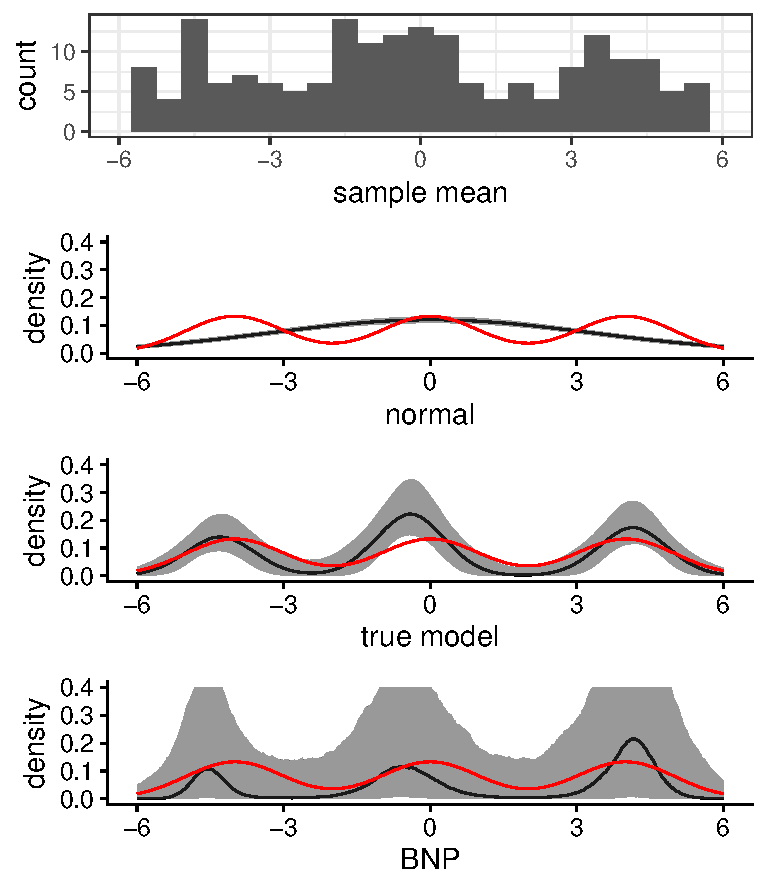
\includegraphics[width=.5\textwidth]{toy_ex/predictive}
\begin{minipage}{.8\textwidth}
\caption{\small Top: Sample averages for simulated data of Section~\ref{subsec:illustration}. The next three rows correspond to pointwise posterior estimates and 90\% credible intervals for the underlying density corresponding to the random distribution, $\mathcal{P}$. For the BNP model, a weighted kernel density estimate employing a bandwidth of 0.1  was used for each posterior draws of $\mathcal{P}$, as the posterior draws do not have a density with respect to Lebesgue measure.}
\end{minipage}
\label{predictive}
\end{figure}


The bottom three panels of Figure \ref{predictive} show density estimates and 90\% pointwise credible intervals based on posterior samples of $\mathcal{P}|y$ for the three models. For the normal model and the ``true" model, these were computed by taking quantiles of the sampled density evaluated on a grid. For the Bayesian nonparameteric model, the sample density was estimated using a weighted kernel with bandwidth of 0.1 because samples of $\mathcal{P}$ do not have a density with respect to Lebesgue measure. The true generating model for the $\mu_g$ is shown in red. The posterior for the density of $\mu_g$ under the normal model has less uncertainty but is concentrated around an incorrect answer because of its inflexibility. Both the "true" and the BNP models contain much of the true density within the pointwise uncertainty intervals. The BNP model shows a great deal more posterior uncertainty because it does not assume a parametric model for $\mu_g$. Despite the increased uncertainty about $\mathcal{P}$, posterior estimation under the BNP model is nearly as good as under the true model; the left panel of Figure~\ref{precision} shows the lengths of the posterior 95\% credible intervals for the $\mu_g$ sorted by their length for the three models; the dotted lines represent correspond to a non-hierarchical analysis (indepedent, uniform priors on $\mu_g$) with $\sigma^2$ known ($+/- 4/\sqrt{3}$). For this data set, we see that both the nonparametric and true models have less posterior uncertainty than the normal model on average, while all three hierarchical models have substantially less uncertainty than a non-hierarchical model. The right panel shows histograms of the mean squared error, $\int (\mu_g - \mu_{g0})^2 p(\mu_g|y) d\mu_g$, computed for each $g$ under the three models, where $\mu_{g0}$ is the true value. Again, we see that estimation is substantially improved when $\mathcal{P}$ is modelled appropriately.

% \begin{figure}[h!]
% 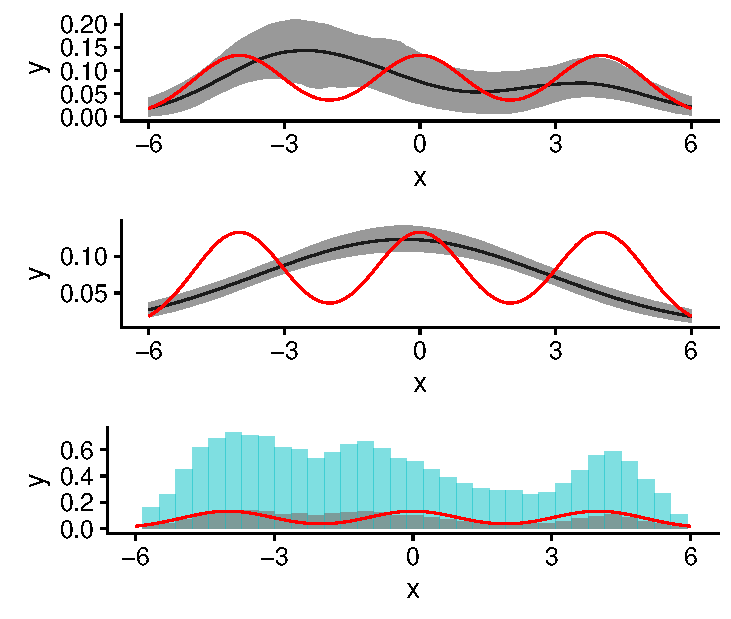
\includegraphics[width=.5\textwidth]{toy_ex/post-pred}
% \caption{Pointwise density estimates for three posterior models based on simulated data of Subsection~\ref{subsec:illustration}}
% \label{ex-predictive}
% \end{figure}

\begin{figure}[h!]
\centering
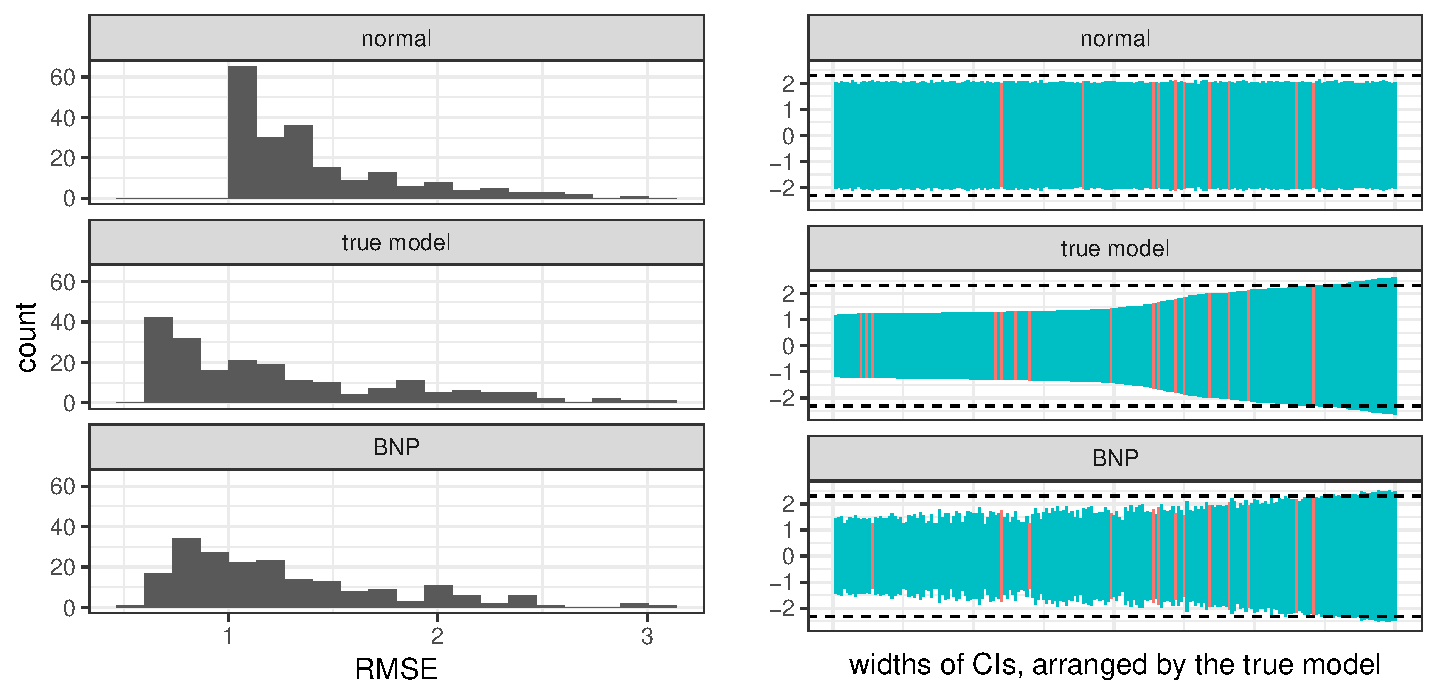
\includegraphics[width=.9\textwidth]{toy_ex/precision}
\begin{minipage}{.8\textwidth}
\caption{\small Left: Histograms of the mean squared error based on posteriors for these models. Right: The widths of the 95\% posterior credible intervals for $\mu_g$ under the three hierarchical models, arranged by the width for the true model. Intervals which failed to cover the true value are colored red. The dashed lines correspond approximately to credible intervals with independent uniform priors on $\mu_g$.}
\end{minipage}
\label{precision}
\end{figure}


\subsection{BNP model for RNA-seq data}
\label{sec:model}
Let $y_{gn}$ represent the normalized log-cpm for gene $g$, sample $n$. Let $x_{n}^\top$ be the row of the design matrix $X$ corresponding to sample $n$. Let $g=1,...,G$ and $n=1,...N$ index genes and samples, respectively. Let
\begin{equation}
y_{gn} \sim \op{N} \left( x_{n}^\top \beta_g, \frac{\sigma^2_g}{w_{gn}} \right)
\end{equation}
where $w_{gn}$ is a given relative precision for $y_{gn}$. While not critical to our method, the inclusion of these precisions allows us to avoid dependence on the assumption of constant variance within genes. This is discussed further in Section \ref{norm-weight}. As discussed in the previous Section, we intend to model the gene-specific parameters nonparametrically, letting the vector of gene specific parameters follow a Dirichlet process. This is denoted by
\begin{equation}
\left(\beta_g^\top,\sigma^2_g\right) \ind \mathcal{P},\quad \mathcal{P} \sim \op{DP}(\alpha \mbox{Q}).
\end{equation}
The Dirichlet process satisfies two requirements proposed by \citet{ferguson} for priors over probability distributions, that it have large support on the space of probability distributions and that it be computationally tractable \citep{ferguson}. The tractibility of the DP is important, because it makes inference computationally feasible. The large support allows us to discard unwarranted parametric assumptions, which can lead to biased inference about $\mathcal{P}$.

The implication is that $\mathcal{P} =\sum_{k=1}^\infty \pi_k \delta_{\left(\tilde{\beta}_k^\top ,\tilde{\sigma}^2_k\right)}$, where $\left(\tilde{\beta}_k^\top ,\tilde{\sigma}^2_k\right) \ind Q$, where $\delta_{x}$ represents the Dirac delta function (a point mass at $x$) and $\pi$ follows a stick-breaking distribution with concentration parameter $\alpha$. The stick-breaking representation of the DP, due to \citet{sethuraman}, is equivalent to a reparameterization of $\{\pi_k\}$ in terms of $\{\nu_k\}$ where $\pi_k = \nu_k \prod_{l<k}(1-\nu_l)$. While the Dirichlet process allows for flexibility in learning $\mathcal{P}$, it can also avoid overfitting the data. These opposing goals are accomplished simultaneously by assuming some positive prior probability that $(\beta_g^\top,\sigma_g^2)=(\beta_{g'}^\top,\sigma^2)$ for any genes, $g$ and $g'$. The stick-breaking distribution is defined by $\nu_k \ind \op{Beta}(1, \alpha),\; \alpha>0$, so that larger values of $\alpha$ will lead to smaller values of $\nu_k$. Notice that $E(\pi_k)=\alpha^{k-1}/(\alpha+1)^{k}$ (because $\nu_k$ are i.i.d.), so $\op{E}(\pi_k)>\op{E}(\pi_l),\;k<l$. It follows that the rate of decay is inversely related to the magnitude of $\alpha$.

The stick-breaking representation of the DP makes clear the role of $Q$: it serves as a kind of proposal distribution for the atoms, $\left(\tilde{\beta}_k^\top ,\tilde{\sigma}^2_k\right)$. We choose $Q$ to be a product measure on the atoms given by
% \iftoggle{thesis}{
% The use of this prior, due to \citet{ferguson}, is a distribution over probability distributions, such that for any finite disjoint partition $\{A_i\}_{i>=1}^n$ on $\mathbb{R}^p$, $\mathcal{P}$ is a random measure such that the joint distribution $\left(\mathcal{P}(A_1),\ldots,\mathcal{P}(A_n)\right) \sim \op{Dir}\left(\alpha Q(A_1),\ldots,\alpha Q(A_n)\right).$ The Dirichlet process has two parameters: $Q$, the base measure, represents a prior guess at the distribution. $\alpha$, the concentration parameter expresses the degree to which $\mathcal{P}$ will agree with $Q$ on any set $A$. This follows from the definition given above and known properties of the Dirichlet distribution, i.e., $\op{E}\left(\mathcal{P}(A)\right)=Q(A)$, and $\op{V}\left(\mathcal{P}(A)\right)=\frac{Q(A)(1 - Q(A)}{\alpha + 1}$, showing that $\mathcal{P}(A) \stackrel{p}{\rightarrow} Q(A)$ as $\alpha \rightarrow \infty$ for any set $A$.
% }{}
% By modeling $\mathcal{P}$ with a Dirichlet process one can be noninformative about the overall shape of $\mathcal{P}$, allowing for irregular shapes, multimodality, and so forth. An argument can be made that by incorporating our uncertainty about these features of the distribution is required for coherent interpretation of the posterior distribution \citep{walker2010bayesian}. For more information about the properties of the DP, see \cite{ferguson}.
%
% As shown by \citet{sethuraman}, it follows from the definition of the Dirichlet process that $\mathcal{P}$ is almost surely discrete and realizations of $\mathcal{P}$ can be produced by the following stick-breaking construction:
%
% Let
% \begin{equation}
% \mathcal{P} =\sum_{k=1}^\infty \pi_k \delta_{\left(\tilde{\beta}_k^\top ,\tilde{\sigma}^2_k\right)}.
% \end{equation}
% Here $\delta_{(.)}$ is the Dirac delta function. Note that although almost sure discreteness is a property applicable to ``draws'' from a DP, the posterior for $\mathcal{P}$ is in fact a mixture of DP \citep{antoniak}. An implication of discretness can be thought of as a ``bet on sparsity"; that there are actually a finite (but unspecified) number of unique values that $(\beta_g^\top,\sigma^2_g)$ can take.
%  The ``atoms" distributed according to $Q$, specified by the product measure

\begin{equation}
\tilde{\beta}_k \sim \op{N}(m_\beta, C_\beta),\quad \tilde{\sigma}^2_k \sim \op{IG}(a_{\sigma^2}, b_{\sigma^2}).
\end{equation}

``$\op{IG}(a,b)$" refers to the inverse gamma distribution which we parameterize by shape and scale parameters, $a$ and $b$ with density given by
\begin{equation*}
p(x|a,b) = \frac{b^a}{\Gamma(a)}x^{a+1}e^{-b/x}.
\end{equation*}


% The mixture weights, $\pi_k$,  follow a stick-breaking process \cite{sethuraman}. Using the reparameterization,
%
% \begin{equation}
% \nu_k = \frac{\pi_k}{1 - \sum_{l=1}^{k-1} \pi_l},
% \end{equation}
%
% $\nu_k$ representing a proportion of the total probability remaining after $k-1$ breaks. For the stick-breaking construction of the DP, the $\nu_k$ are modeled by:
% \begin{equation}
% \nu_k \ind \op{Beta}(1, \alpha).
% \end{equation}
%
% This assumption induces a stochastically decreasing ordering of the weights. Additionally, note that $\sum_{k=1}^K \pi_k \stackrel{p}{\rightarrow} 1$ as $K\rightarrow \infty$.

\subsection{Normalization and precision weights}
\label{norm-weight}
\paragraph{Between sample normalization}
Artifacts of the sequencing procedure can lead to some samples having larger or smaller read counts on average relative to other sample. This introduces biases that require adjustment. These corrections are typically made at the time of analysis by introducing a sample specific offset. Different methods for normalization have been proposed. \citet{robinson2010} proposed a method called trimmed mean of M-values (TMM) to correct between-sample biases by compare observed log-fold-change values between samples for all genes. Under the assumption that most genes are not differentially expressed, they use a trimmed mean to robustly estimate the bias. When there are more than two samples, the same methodology is extended by using one sample as a reference. For details, see \citet{robinson2010}.

\paragraph{Precision weights adjust for non-constant variance}
Theory suggests that an RNA-seq count, $C$, would have a Poisson distribution, with variance equal to the mean ($\op{Var}(C_{gn})=\op{E}(C_{gn})=\mu_{gn}$, if the RNA from the same sample were sequenced repeatedly. Biological variation (either between subjects or through repeated sampling) leads to overdispersion of the counts. Often, the negative binomial distribution is used to allow for variance that is quadratic with the mean ($\op{Var}(C_{gn})=\mu_{gn}+\phi_g\mu_{gn}^2$). Because gene expression is usually measured on the log scale, consider the delta method  approximation for a negative binomial count in terms of the log-count: $\op{Var}(\log C_{gn}) \approx (1/\mu_{gn})^2(\mu_{gn} + \phi_g\mu_{gn}^2)=1/\mu_{gn} + \phi_g$. In other words, for a fixed $\phi>0$, a negative binoimal assumption assumes log-counts whose variance is a decreasing function of the mean, with asymptote at $\phi_g>0$. Empirical evidence \citep{voom} suggests that the overdispersion parameter, $\phi_g$, tends to be larger for genes with lower expression than those with higher expression. Unlike the normal distribution, the negative binomial distribution with unknown dispersion parameter is not an exponential family and is less computationally convenient to work with.

\cite{voom} proposed a method called \textit{voom}, as a way to make RNA-seq data compatible with normal linear models. \textit{voom} introduces count specific precision weights, estimated from the all of the data, to compensate for the non-constant mean-variance relationship present in RNA-seq. Briefly, first a regression computed for each gene, producing a standard deviation and mean log-count. Next a smooth nonparametric regression is fit to the square root of the gene-wise standard deviations, using the mean log-counts as a predictor. The weights are then estimated using this fitted model. This procedure implies that the variance of a count is given by, $\op{Var}(\log C_{gn})=\sigma_{g}^2\op{Var}_{LOWESS}(\mu)$. We use \texttt{voom} in our pipline by estimating $\op{Var}_{LOWESS}(\mu)$ and plugging in preliminary estimates of $\mu_{gn}$ to get $w_{gn} = \widehat{\op{Var}}_{voom}(\hat{\mu}_{gn}).$

Rather than assuming the mean-variance relationship of the negative binomial and allowing for an adjustment of the degree of overdispersion from gene to gene, voom's precision weighting scheme estimates the mean-variance relationship from the data and assumes that it applies both within as well as across genes. We use the precision weights as an input to our model (Section \ref{sec:model}) which estimates a gene-specific variance parameter. Our use of voom in our pipeline implies a gene-specific mean-variance relationship \textit{for the log counts} given by
$$\op{V}(\log C|\mu)=\sigma^2_g \widehat{\op{V}_{voom}(\log C|\mu)}.$$

\subsection{Priors}
The base measure, $Q$, represents a prior guess at $\mathcal{P}$. The use of diffuse base measures is not recommended as it can result too few practically significant weights, $\pi_k$ \citep[p.554]{gelman-book}. For purposes of comparability, we used the \texttt{estimateBetaPriorVar} function from the \texttt{DESeq2} package to set $Q$. This function chooses variances to match the quantiles of the empirical distribution of the independently obtained estimates of $\beta_g$, $\sigma_g^2$. The prior distribution for $\alpha$ was chosen by considering the implied expected number of clusters. Although is difficult to guess the number of clusters \textit{a priori}, we believe that most genes will have a pattern of expression that is similar to some other gene, so that after grouping the genes into clusters, the number of clusters should be much smaller than the number of genes. Also, due to computational constraints, we cannot deal with more than about 6000 clusters. Based on these considerations, we select the prior $\alpha \sim \op{Ga}(3,3/G^{0.5})$, which implies the expected number of clusters is likely between $G^{0.5}$ and $G^{0.75}$.

%For $\beta_gl$; $l=2,3,4,5$, these were obtained using the \texttt{estimateBetaPriorVar} from the \texttt{DESeq2} package using the ``quantile" method. For $\beta_g1$ and $\sigma^2_g$, a similar m

\subsection{Gibbs Sampler}
Our Gibbs sampler for performing MCMC sampling from the posterior distribution for the BNP model is adapted from the blocked Gibbs sampler of \citet{ishwaran2000}. The steps are as follows:

\paragraph{Sample $\zeta_g$, $\alpha$:}

\begin{equation*}
\zeta_g \ind \op{Categorical}\left(\hat{\pi}_1,\ldots,\hat{\pi}_K \right), \mbox{ with}
\end{equation*}
\begin{equation*}
\hat{\pi}_k \propto \pi_k \op{N}(y_g;X\tilde{\beta}_k,\tilde{\sigma}_k^2 W_g).
\end{equation*}
Here $W_g$ is a diagonal matrix consisting of the log-count specific precisions. Conditional on everything else, the $\zeta_g$ parameters are independent $K$-categorical random variables with weights proportional to the likelihood of $y_g$ given $\tilde{\beta}_k$ and $\tilde{\sigma}_k$, weighted by $\pi_k$. This step is the most computationally intensive; just computing the weights requires the calculation of $G\times K$ such likelihoods. However, using fine-grained GPU parallelism, doing so is practically feasible. $\alpha$ is conditionally independent of the $\zeta_g$s and has the conjugate full conditional
\begin{equation*}
\alpha \sim \op{Gamma}(K + a_\alpha - 1, -\log \pi_K + b_\alpha).
\end{equation*}


\paragraph{Sample $\tilde{\beta}_k$:}
\begin{equation*}
\tilde{\beta}_k \sim \op{N}(\hat{m}_k,\, \hat{C}_k),
\end{equation*}
\begin{equation*}
\mbox{ where }\hat{C}_k= \left( \sigma^{-2}_g\sum_{g:\zeta_g=k}
  X^\top W_g X + C^{-1} \right)^{-1}, \mbox{ and }\hat{m}_k=\hat{C}_k \left(\sum_{g:\zeta_g=k} X^\top W_g y_g +
      C^{-1}m \right).
\end{equation*}
The $\tilde{\beta}_k$ are conditionally independent. Note that if $\zeta_g \neq k$ for all $g$, then $\tilde{\beta}_k$ is simply drawn from it prior.

\paragraph{Sample $\tilde{\sigma}_k^2$s}
\begin{equation*}
      \tilde{\sigma}_k^2 = \op{IG}(\hat{a}_k,\hat{b}_k),
    \end{equation*}
    \begin{equation*}
      \mbox{ where }\hat{a}_k = a_{\sigma^2} + \frac{1}{2}NM_k,\mbox{ and }\hat{b}_k= b_{\sigma^2} + \frac{1}{2}\sum_{g:\zeta_g=k}y_g^\top W_g y_g -2 \beta_g^\top X^\top W_g y_g  +\beta_g^\top X^\top W_g X \beta_g
    \end{equation*}

    Here $M_k$ is the number of $g$ for which $\zeta_g = k$. Again, the $\tilde{\sigma}_k$ are conditionally independent.

\paragraph{Sample $\nu$}
\begin{equation*}
\nu_k ~ \op{Be}(M_k + 1, \sum_{l>k}M_l + \alpha).
\end{equation*}

Given $\alpha$ and $\zeta$, the $\nu_g$ are conditionally independent. Derivations of the full conditionals are given in the Appendix.

\section{Simulation study 1}
Since the proposed BNP method uses voom weights, we did a simulation study to compare the our method to the voom-limma method for RNA-seq data. The voom-limma method fits a linear model to the data under the same transformation conditional on the same voom quality weights, but proceeds by fitting each gene independently. Thus, a comparison of the estimates obtained under BNP model to the voom-limma estimates will show the result of borrowing information across genes via the Dirichlet process prior on $\mathcal{P}$.

\begin{table}
\caption{Data simulation procedure for Simulation study 1}
\begin{enumerate}
\item Select random draw of $\mathcal{P}$, $\mathcal{P}^{(s)}$, obtained from the posterior distribution given the entire Paschold data set
\item Sample $(\beta_g,\sigma^2_g)$ independently from $\mathcal{P}^{(s)}$, $g=1,\ldots,10000$
\item Sample $y_{g} \sim N(X\beta_g,\sigma^2_g I)$
\end{enumerate}
\end{table}
% Produce 6-10 such data sets\\

\paragraph{TREAT}
A common goal of gene expression profiling is to produce a ranked list of 'called' genes for which a particular hypothesis is most likely to be true. The authors of \texttt{limma} provide multiple methods for calling genes. One method, called a TREAT, tests whether the log-fold-change due to a model term is larger than a specified threshold in absolute value, i.e. it allows users to ranking genes based on the evidence of the hypothesis, $H_{gl}:|\beta_{gl}|>t$. The inclusion of this test in their software was in response to the observation that even if an effect is statistically significant, often it is uninteresting unless it has a certain magnitude. TREAT is a moderated t-test that involves an shrunken estimates of $\sigma^2_g$ \citep{treat}. For more details, see \citet{treat}.

We can compare the ranking given by \texttt{limma} to ones based on posterior probabilites that $H_{gl}$ is true. We use receiver operating characteristic (ROC) curves to do this. ROC curves provide a graphical summary of the performance of a classifier by showing, as a function of the top $H$ genes as ranked by the classifier, the the proportion of cases correctly identified (true positive rate, TPR) along with the proportion of non-cases that are improperly identified (false positive rate, FPR). The top panel of Figure \ref{roc-ss1} shows a typical receiver operator characteristic curve among the ten we observed. The bottom panel shows the area under the ROC curve (AUC) up to a FPR of 0.1. For both plots we show results for each component of $\beta$ (excluding the intercept) and a range of thresholds. In our simulations the BNP method tended to outperform \texttt{limma} on average. Note that while \texttt{limma} can perform tests with a threshold of zero, there is no comparable result for the BNP model, since this hypothesis has probability zero. The exception seems to be for the parental half-difference. For that particular set of tests, both \texttt{limma} and BNP appear to have similar accuracy.
%The comparative advantage seems to depend on the threshold: When $t=0$, there is little difference in the ROCs for testing $H_{g3}$, but as the threshold was increased to a log-fold change of 0.2, BNP outperformed \texttt{limma} by a wide margin.
% This suggests that our method, by ``learning" the underlying distribution of $\beta$, increases the ability to detect effects of practical significance.
% 
\begin{figure}[ht!]
\centering
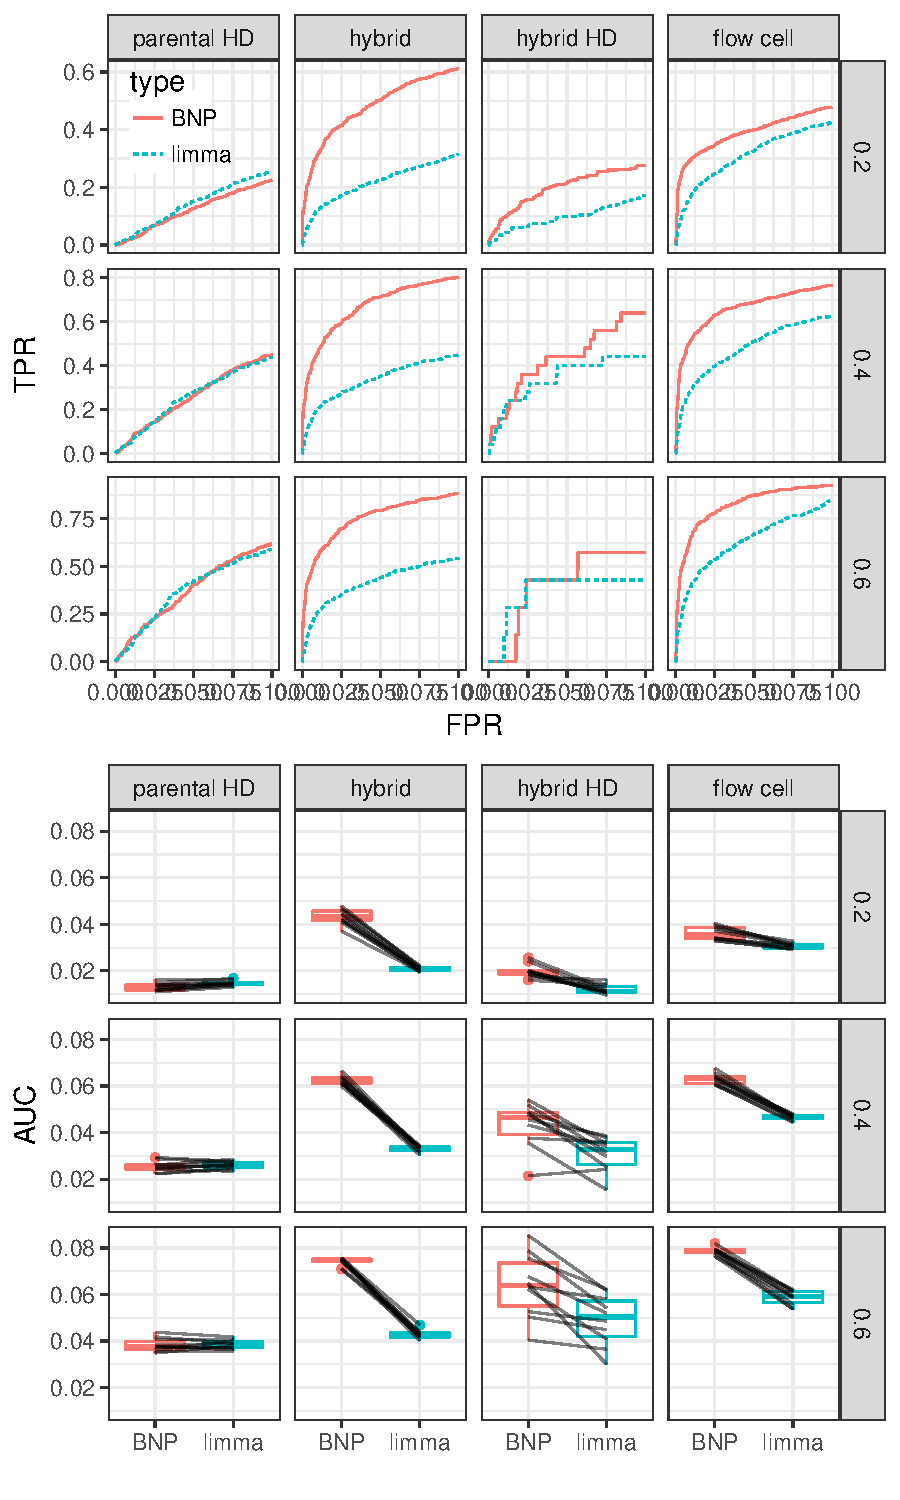
\includegraphics[height=.8\textheight]{ss1-roc-auc}
\caption{ROC curves for a typical simulation and AUC for testing whether absolute effect sizes exceed a threshold for various thresholds for simulation study 2. Comparison is made between BNP and limma.}
\label{roc-ss1}
\end{figure}

We also compared the accuracy of point estimate under the two models. Here we expect BNP to do much better than \texttt{limma}. This is because \texttt{limma} produces point estimates for $\beta_g$ without any pooling, whereas the BNP provides shrinkage toward the mass of the underlying distribution of the $\beta_g$s. Figure \ref{mspe-ss1} shows that this is indeed the case; the mean squared prediction errors averaging across genes are uniformly smaller that those for \texttt{limma}.

\begin{figure}[ht!]
\centering
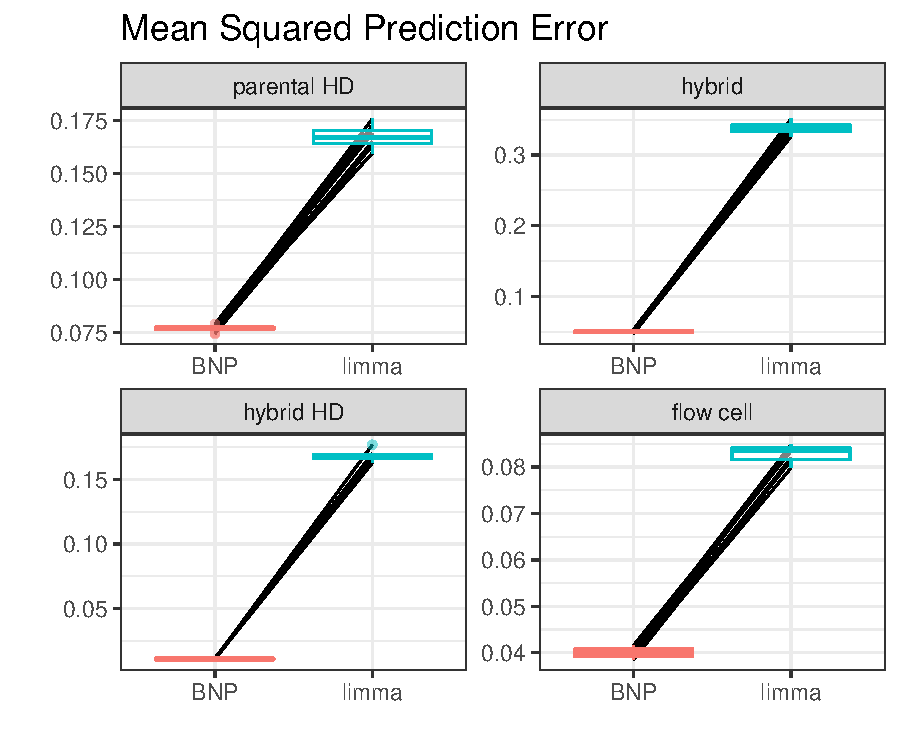
\includegraphics[width=.8\textwidth]{ss1-mspe}
\begin{minipage}{.8\textwidth}
\caption{\small Mean squared prediction error for each effect for simulation study 1. Comparison is made between BNP and limma.}
\end{minipage}
\label{mspe-ss1}
\end{figure}

\section{Simulation study 2}
Much of the recent methods proposed for the analysis of RNA-seq data are based on an assumption that repeated sequencing of the same sample would produce Poisson distributed counts. For example, \cite{mccarthy} motivates the negative binomial model by showing that it has the right mean-variance relationship given the the above assumption and an assumption that the coefficient of variation is for constant within a gene. A popular approach is to use a negative binomial generalized linear model with log link function.

To compare estimation and accuracy of gene selection with existing methods designed for RNA-seq count data, we simulated count data by fitting the Paschold data with \texttt{voom/limma} and sampling a random subset of 10,000 genes without replacement. We then simulated normal data, conditioning on the estimates of $\beta_g$, $\sigma^2_g$, as well as the estimated precision weights. These simulated log-cpm values were then converted to log-counts, centering by $\log_2(\bar{R}_\cdot)-\log_2(10^6)$, where $\bar{R}_\cdot$ is the geometric mean of the estimated effective library sizes. Finally, these log-counts ($y_{gn}$) were exponentiated and rounded to obtain the simulated counts, $C_{gn}$. For each simulated data set, we analyzed the data using our BNP method and also with two popular count-based methods, \texttt{edgeR} and \texttt{DESeq2}, the latter both with and without independent normal priors on the $\beta$s \citep{edger2010,deseq2014}. For purposes of comparison, we considered accuracy of point estimation via mean squared prediction error and accuracy in identifying interesting genes using ROC curve.
\begin{table}
\caption{Data simulation procedure for Simulation study 2}
\begin{enumerate}
\item Sample 10,000 indices, $g$, from $\{1,2,\ldots,36,000\}$ without replacement.
\item Set $\beta_g:= \hat{\beta}_{voom,~g},\; \sigma^2_g:= \hat{\sigma}^2_{voom,~g}$
\item Sample $y_{gn} \sim \op{N}(x{gn}^\top\beta_g, \sigma^2_g/w_{gn})$
\item Set $C_{gn} = \op{Round} \left\{ 2^{y_{gn} + \log_2(10^6) - \log_2(\bar{R}_{\cdot})} \right\}$
\end{enumerate}
\end{table}


% Ranking accuracy (ROCs)
Both \texttt{edgeR} and \texttt{DESeq2}  provide threshold tests similar to TREAT in \texttt{limma}. We again used ROC to compare the accuracy in gene ranking between these three methods. For this simulation, unlike the first, the true parameters for each gene are unique. In general, the difference in performance was less noticable in this simulation. To get at a measure of overall performance, we calculated the area under the ROC curve (AUC) up to a false positive rate of 0.1. Comparing AUC across the ten simulations (Figure \ref{ss2-roc}), we see that there were difference is rankings between the methods for different tests and thresholds. BNP appears to do nearly as well as both \texttt{DESeq2} methods and \texttt{edgeR} under each condition. Interestingly, \texttt{DESeq2} with normal priors for $\beta$ does poorest overall, particularly when testing for hybrid and hybrid half-difference affects above a threshold. Because the data are least informative about these two affects and many are likely near zero, it is likely that the prior is too informative, shrinking these toward zero. The BNP was more accurate in identifying genes with hybrid affects where the log-fold change was greater than a threshold. We think that BNP does better here because the parental half-difference is informative about the hybrid affect, which is captured in the posterior for $\mathcal{P}$. We discuss this further in Section \ref{analysis}. A comparison of the mean squared prediction error in the point estimates for $\beta$ is more definitive 

\begin{figure}[ht!]
\centering
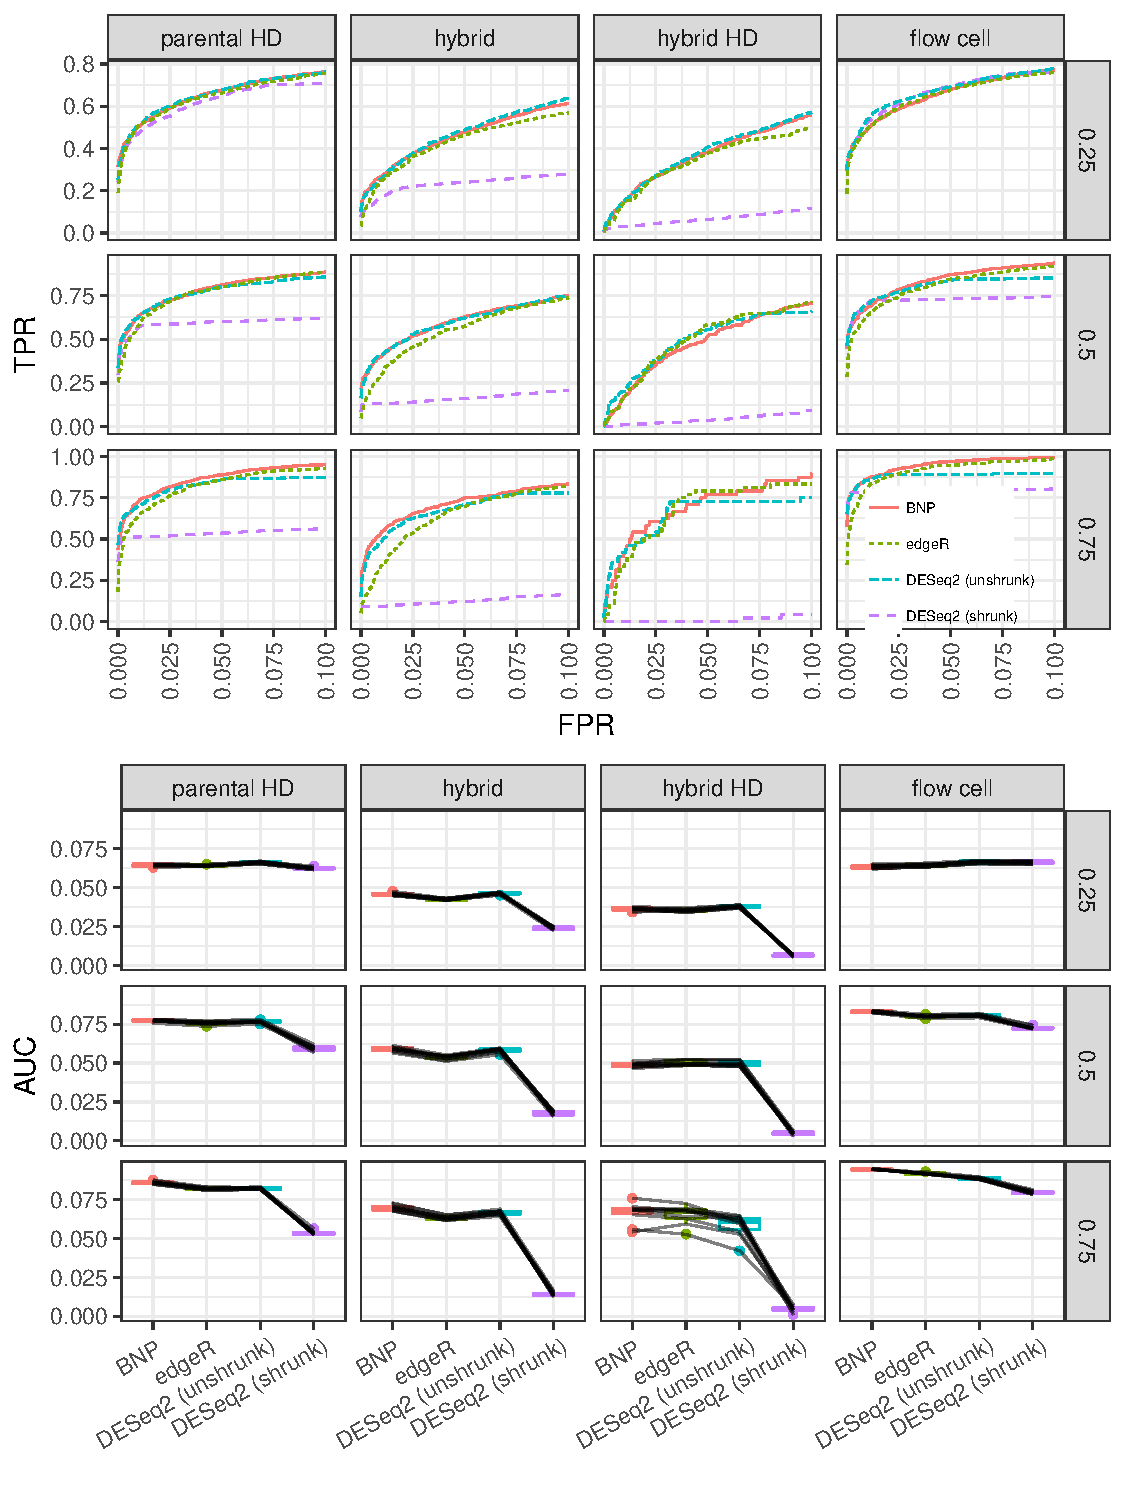
\includegraphics[height=.8\textheight]{ss2-roc-auc2}
\begin{minipage}{.8\textwidth}
\caption{\small ROC curves for a typical simulation and AUC for testing whether absolute effect sizes exceed a threshold for various thresholds for simulation study 2. Comparison is between BNP, edgeR and DESeq2 with and without independent normal priors for $\beta$.}
\end{minipage}
\label{ss2-roc}
\end{figure}

% Mean squared prediction error
For each simulation we computed the mean squared prediction error (MSPE) corresponding to each element of $\beta_g$, $\frac{1}{G}\sum_{g=1}^G (\hat{\beta}_g-\beta_g)^2$ for both methods. The results, shown in Figure \ref{ss2-mspe}, show the comparison between BNP is more accurate with respect to MSPE than both \texttt{DESeq2} and \texttt{edgeR}.

\begin{figure}[ht!]
\centering
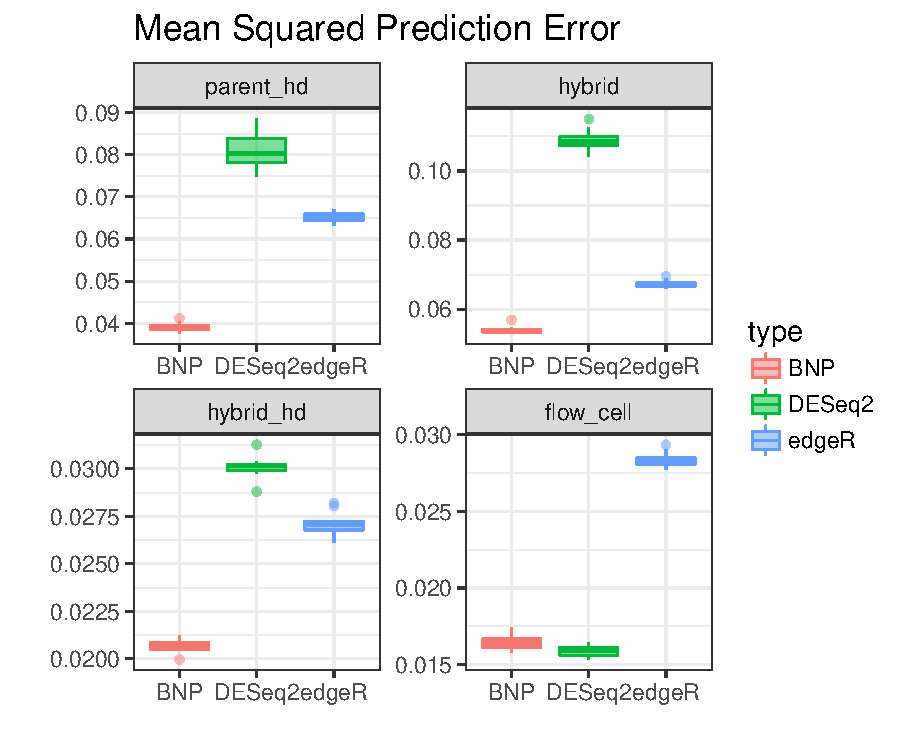
\includegraphics[width=.8\textwidth]{ss2-mspe}
\begin{minipage}{.8\textwidth}
\caption{\small Comparing the accuracy of estimation of $\beta_g$ for BNP, edgeR and DESeq2. Results show the average squared prediction error for 10 simulated data sets.}
\end{minipage}
\label{ss2-mspe}
\end{figure}


A further advantage that we have over these other methods is that by using posterior samples, we can evaluate probabilites of hypotheses with composite null parameter spaces which cannot be done using these other packages.
%\citet{wang-phd} discussed how the geometry of the null parameter space for heterosis leads to serious difficulties with classical likelihood ratio tests; not the least of which is that p-values are not uniformly distributed under the null hypothesis, invalidating assumptions needed to apply corrections for multiple testing.

\begin{table}
\caption{Definition of types of gene heterosis in terms of mean expression by genotype as well as using parameterization implied by the design matrix.}
\label{def-heterosis}
\begin{tabular}{ccc}
Type of heterosis & Relation & $\beta$-parameterization\\
high-parent B73xMo17 & $\max\{\mbox{B73,Mo17}\} < \mbox{B73xMo17}$ & $\phantom{-}|\beta_{g2}| < \beta_{g3} + \beta_{g4}$\\
low-parent B73xMo17  & $\min\{\mbox{B73,Mo17}\} > \mbox{B73xMo17}$ & $-|\beta_{g2}| > \beta_{g3} + \beta_{g4}$\\
high-parent Mo17xB73 & $\max\{\mbox{B73,Mo17}\} < \mbox{Mo17xB73}$ & $\phantom{-}|\beta_{g2}| < \beta_{g3} - \beta_{g4}$\\
low-parent Mo17xB73  & $\min\{\mbox{B73,Mo17}\} > \mbox{Mo17xB73}$ & $-|\beta_{g2}| > \beta_{g3} - \beta_{g4}$
\end{tabular}
\end{table}

The ROC plots suggests that the posterior probabilites do a good job with ranking the genes. However, because they are interpretable as probabilites, we can still question their accuracy relative to the frequency of true positives. Figure \ref{calib-ss2} shows estimated calibration curves for the 10 simulation studies for a set of hypotheses that might be of interest to researchers. Each curve was produced by binning genes by binning genes with similar posterior probabilites and plotting relative frequency of ``true-positives" vs. the midpoint probability of the bin. Note that monotonicity in the probabilities when sorted by true conditionis all that is needed to produce a good ROC.

\begin{figure}[ht!]
\centering
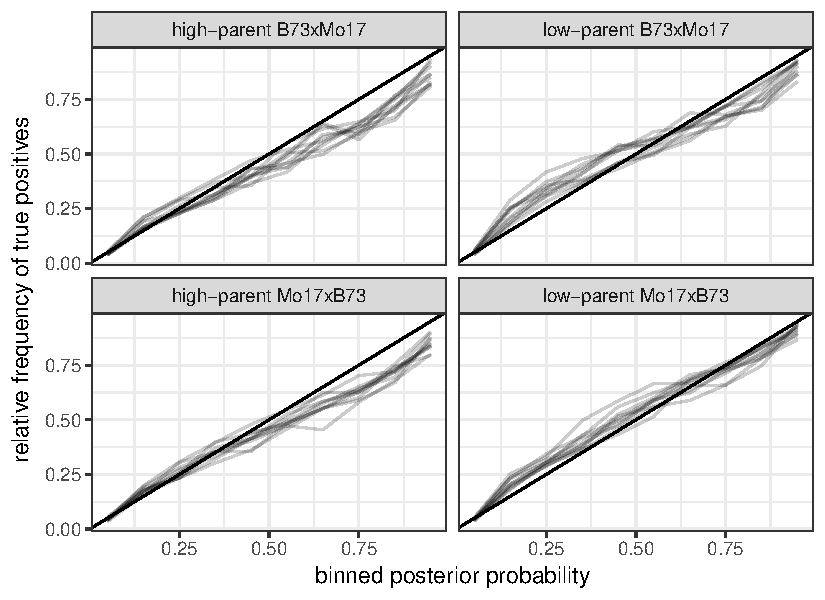
\includegraphics[width=.8\textwidth]{calib-ss2}
\begin{minipage}{.8\textwidth}
\caption{\small Calibration curves for BNP posterior probabilities for simulation study 2. Curves were constructed by binning posterior probabilities into equal width intervals. The midpoint of the interval was used for plotting on the x-axis and the y-axis shows the true frequency of genes for which the hypothesis is true.}
\end{minipage}
\label{calib-ss2}
\end{figure}

\section{Analysis of Paschold data}
\label{analysis}
To fit the Paschold data, we ran 4 chains, each for 40,000 iterations after 30,000 iterations of warmup. The samples were thinned by a factor of 40, for a total of 4,000 thinned post-warmup draws for each gene-specific parameter and $\alpha$. Posterior probabilities of prespecified hypotheses as well as posterior means and meansquares for the gene-specific parameters, $\beta_g$ and $\sigma_g$, were computed using all the draws using running means.

In the original paper, a the results of a set of hypothesis tests was used to classify genes into nine categories specifying the relationships between mean expression of each hybrid variety and the two parental lines. In Figure \ref{orig-compare}, we show histograms of posterior probabilities pertaining to high- and ow-parent gene heterosis for the genes subsetted by whether or not they were classified as ``discoveries'' in the original paper. High-parent heterosis corresponds to genes for which the mean expression of the hybrid is higher than the more highly expressed parent and low-parent heterosis where it is lower than the less expressed parent. Generally speaking, the posterior probabilities tend to agree with the categorization --- particularly for non-discoveries --- however, a number of discoveries have low posterior probabilities in our analysis. This is likely due to borrowing of information across genes leading to shrinkage toward general patterns of expression, where both low- and high- parental expression were uncommon (\citet{paschold} found evidence of these extreme patterns in less than 1\% of genes.) We also note that a small number of non-discoveries are found to have high-posterior heterosis probabilities. Due to the multidimensional shrinkage featured by the model, it can be difficult to sort out what accounts for the difference in some cases.

\begin{figure}[h!]
\centering
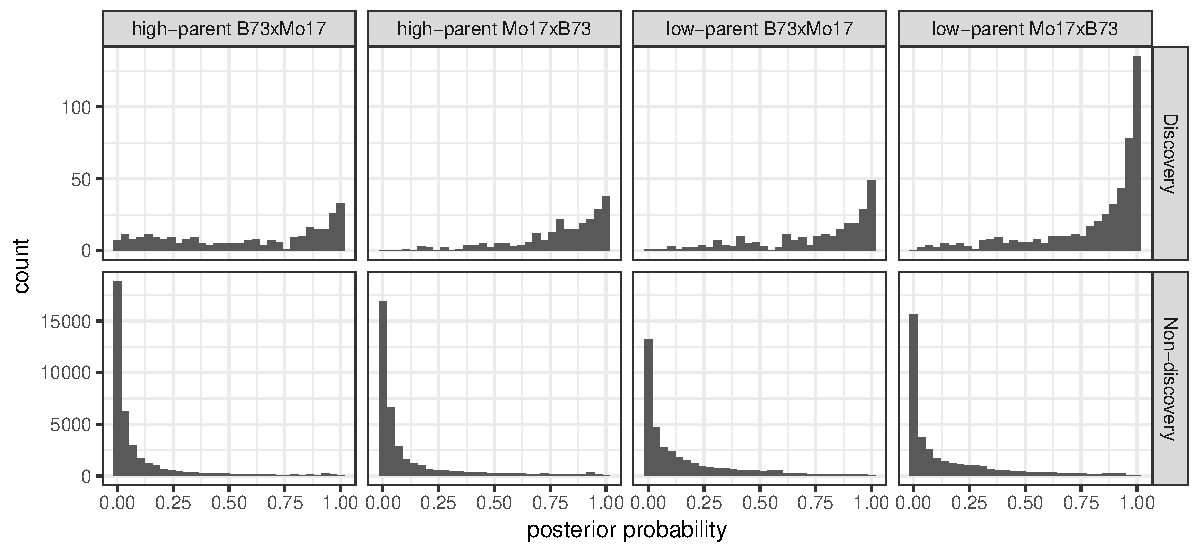
\includegraphics[width=\textwidth]{orig-compare}
\begin{minipage}{.8\textwidth}
\caption{\small Posterior probabilities for low- and high-parent gene heterosis hypotheses for subsets of genes classified as discoveries and non-discoveries in the original article (Paschold et al. 2012).}
\end{minipage}
\label{orig-compare}
\end{figure}

Figure \ref{het-shrink} shows how the nonparametric model shrinks estimates. Genes categorized as showing evidence of extreme gene heterosis in the original paper are represented as black points. The left panel shows independently obtained estimates for the parental half-difference and the mean hybrid effect overlayed on a bivariate histogram of the independent estimates for all genes. The right
panel shows the corresponding estimates for our analysis overlayed on a posterior pointwise estimate of $\mathcal{P}$. In this second plot we can see significant shrinkage toward the regions where $\mathcal{P}$ has higher posterior density. This helps to explain why a large number of discovered genes have low posterior probabilities for the heterosis hypotheses: when weighed against the overall patterns within the data, in many cases it is likely that the magnitude of the independent estimates is overstated and that detection was a result of random variation.

A result of this shrinkage is increased posterior precision. Figure \ref{exemplars} shows 90\% posterior credible intervals for the exemplar genes from Table \ref{counts}.

\begin{figure}[ht!]
\centering
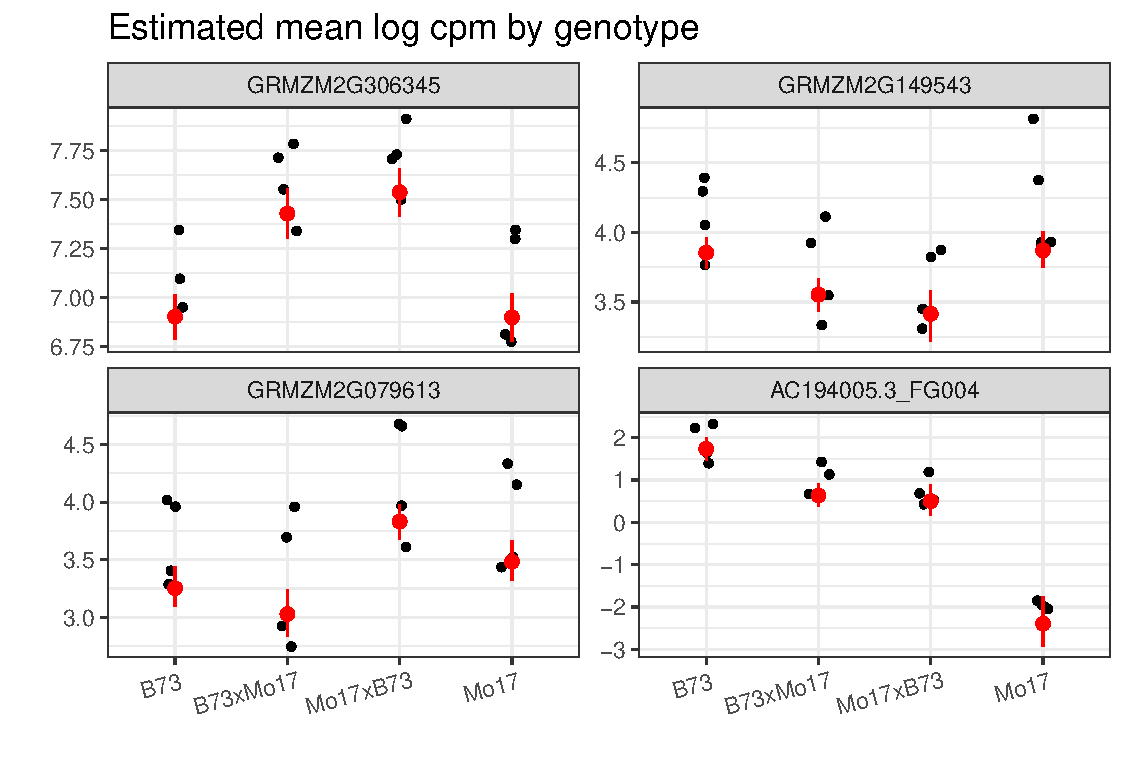
\includegraphics[width=.7\textwidth]{exemplars}
\begin{minipage}{.8\textwidth}
\caption{\small Plots of the exemplar genes from Table \ref{counts}, illustrating presence and absence of patterns of heterosis. The points are jittered horizontally and displayed on the scale of log counts per million. The uncertainty intervals shown are 90\% credible intervals from the fitted BNP model.}
\end{minipage}
\label{exemplars}
\end{figure}

\citet{landau2016high} undertook an analysis of the same data. They modeled the counts directly as Poisson, using a generalized linear model with log link and gene-specific linear predictors as well as a gene-specific overdispersion parameter. It is interesting to compare their results to ours as their method was also fully Bayesian. They assumed independence in the distribution of the linear predictors. Table \ref{bayes-compare1} shows a comparison of the posterior probabilities found by our method to Landau's binned into five intervals for each of the four types of extreme heterosis. While there is a fair amount of agreement between these two methods on the genes with highest and lowest probabilities of heterosis, the differences between the inferences are considerable.

% latex table generated in R 3.4.2 by xtable 1.8-2 package
% Tue Nov 14 21:58:47 2017
\begin{table}[ht]
\footnotesize
\centering
\caption{Two-way tables comparing the posterior probabilities of low-parent gene heterosis for all genes in the Paschold (2012) data set found by BNP and Landau (2016).}
\label{bayes-compare1}
% % \begin{tabular}{rrrrrr}
% % &  &\multicolumn{4}{c}{Landau}\\
% %   \toprule
% % & & [0,0.25] & (0.25,0.5] & (0.5,0.75] & (0.75,1] & total\\
% %   \midrule
% % \multirow{4}{*}{BNP} & [0,0.25] & 20435 & 5499 & 1687 & 702 \\
% %   & (0.25,0.5] & 1299 & 1978 & 930 & 550 \\
% %   & (0.5,0.75] & 446 & 1115 & 486 & 509 \\
% %   & (0.75,1] & 148 & 287 & 167 & 583 \\
% %   & total
% %    \bottomrule
\begin{tabular}{rrrrrrr|r}
&  &\multicolumn{6}{c}{Landau (2016)}\\
  \toprule
&  & [0,0.05] & (0.05,0.15] & (0.15,0.85] & (0.85,0.95] & (0.95,1] & total \\
  \midrule
\multirow{6}{*}{BNP} & [0,0.05]    & 0.283 & 0.083 & 0.116 & 0.001 & 0.000 & 0.483 \\
                     & (0.05,0.15] & 0.017 & 0.037 & 0.129 & 0.003 & 0.001 & 0.186 \\
                     & (0.15,0.85] & 0.009 & 0.025 & 0.254 & 0.017 & 0.009 & 0.313 \\
                     & (0.85,0.95] & 0.000 & 0.000 & 0.007 & 0.002 & 0.002 & 0.011 \\
                     & (0.95,1]    & 0.000 & 0.000 & 0.003 & 0.001 & 0.003 & 0.007 \\
                     \midrule
                     & total       & 0.308 & 0.145 & 0.508 & 0.022 & 0.016 & 1.000 \\
   \bottomrule
\end{tabular}
\\[.5cm]
Low-parent heterosis B73$\times$Mo17.
\\[.75cm]

% \begin{tabular}{rrrrrr}
% &  &\multicolumn{4}{c}{Landau}\\
%   \toprule
% & & [0,0.25] & (0.25,0.5] & (0.5,0.75] & (0.75,1] \\
%   \hline
% \multirow{4}{*}{BNP} & [0,0.25] & 21486 & 4557 & 1486 & 677 \\
%  &  (0.25,0.5] & 1639 & 2155 & 611 & 306 \\
%  &  (0.5,0.75] & 301 & 989 & 522 & 390 \\
%  &  (0.75,1] & 140 & 677 & 197 & 688 \\
%    \bottomrule
   \begin{tabular}{rrrrrrr|r}
&  &\multicolumn{6}{c}{Landau (2016)}\\
  \toprule
&  & [0,0.05] & (0.05,0.15] & (0.15,0.85] & (0.85,0.95] & (0.95,1] & total \\
  \midrule
\multirow{6}{*}{BNP} & [0,0.05] & 0.296 & 0.090 & 0.135 & 0.003 & 0.001 & 0.523 \\
                     & (0.05,0.15] & 0.021 & 0.036 & 0.093 & 0.002 & 0.001 & 0.152 \\
                     & (0.15,0.85] & 0.010 & 0.031 & 0.237 & 0.011 & 0.005 & 0.295 \\
                     & (0.85,0.95] & 0.000 & 0.000 & 0.015 & 0.002 & 0.003 & 0.021 \\
                     & (0.95,1] & 0.000 & 0.000 & 0.003 & 0.002 & 0.005 & 0.010 \\
                     \midrule
                     & total & 0.327 & 0.157 & 0.483 & 0.020 & 0.014 & 1.000 \\
   \bottomrule
\end{tabular}
\\[.5cm]
Low-parent heterosis Mo17$\times$B73.
\end{table}

\begin{table}[ht]
\footnotesize
\centering
\caption{Two-way tables comparing the posterior probabilities of high-parent heterosis for all genes in the Paschold (2012) data set found by BNP and Landau (2016).}
\label{bayes-compare2}
   \begin{tabular}{rrrrrrr|r}
&  &\multicolumn{6}{c}{Landau (2016)}\\
  \toprule
&  & [0,0.05] & (0.05,0.15] & (0.15,0.85] & (0.85,0.95] & (0.95,1] & total \\
  \midrule
\multirow{6}{*}{BNP} & [0,0.05] & 0.395 & 0.126 & 0.155 & 0.000 & 0.000 & 0.676 \\
                     & (0.05,0.15] & 0.037 & 0.037 & 0.085 & 0.000 & 0.000 & 0.159 \\
                     & (0.15,0.85] & 0.020 & 0.025 & 0.100 & 0.003 & 0.001 & 0.149 \\
                     & (0.85,0.95] & 0.000 & 0.000 & 0.011 & 0.001 & 0.001 & 0.012 \\
                     & (0.95,1] & 0.000 & 0.000 & 0.003 & 0.001 & 0.001 & 0.005 \\
                     \midrule
                     & total & 0.452 & 0.187 & 0.353 & 0.005 & 0.002 & 1.000 \\
   \bottomrule
\end{tabular}
\\[.5cm]
High-parent heterosis B73$\times$Mo17.
\\[.75cm]

\begin{tabular}{rrrrrrr|r}
&  &\multicolumn{6}{c}{Landau (2016)}\\
  \toprule
&  & [0,0.05] & (0.05,0.15] & (0.15,0.85] & (0.85,0.95] & (0.95,1] & total \\
  \midrule
\multirow{6}{*}{BNP} & [0,0.05] & 0.352 & 0.115 & 0.165 & 0.000 & 0.000 & 0.633 \\
                     & (0.05,0.15] & 0.035 & 0.032 & 0.087 & 0.000 & 0.000 & 0.155 \\
                     & (0.15,0.85] & 0.033 & 0.035 & 0.116 & 0.005 & 0.002 & 0.190 \\
                     & (0.85,0.95] & 0.001 & 0.001 & 0.014 & 0.001 & 0.001 & 0.017 \\
                     & (0.95,1] & 0.000 & 0.000 & 0.003 & 0.001 & 0.001 & 0.005 \\
                     \midrule
                     & total & 0.421 & 0.183 & 0.386 & 0.007 & 0.003 & 1.000 \\
   \bottomrule
\end{tabular}
\\[.5cm]
High-parent heterosis Mo17$\times$B73.
\end{table}


From the marginal distributions of probabilities, we see that BNP finds lower chances of LPH across genes than Landau. For example, Landau found 1.6\% of genes to have greater than 95\% probability of low-parent heterosis for B73$\times$Mo17, but the majority of these were given less than 85\% probability by BNP. However, BNP also found higher probabilities for some genes: More than 1/3 of the 0.7\% genes which BNP found to be high probablity genes ($>$95\%) were found to only have moderate probabilities (15\%-85\%). The story is different for HPH. Here, BNP has greater confidence, finding both more high- and low-probability genes than Landau.

While we cannot say from these comparisons whether one model is better than another, they serve to highlight the impact that distributional assumptions can have in detecting patterns of gene expression. Given our belief that models like that of \citet{landau2016high} and \citet{deseq2014} make unreasonable assumptions about the distribution of the gene-specific parameters, we expect that the BNP probabilites incorporate more information about the broader patterns of expression exhibited in the data.

\iftoggle{thesis}{
On a different note, \citet{landau2016high} found that when an independent normal model was assumed for $\beta_{gl}$, their posterior distributions were well approximated by a normal distribution matching the first two posterior moments. This is convenient because computation of these moments requires minimal storage, as running means can be used to update these after each iteration of the MCMC chain.

Figure \ref{compare-to-approx} shows full posterior distributions and normal approximations for each component of $\beta_g$ for four randomly selected genes. The quality of the moment-based approximation is satisfactory in some cases but not in others. Due to the discrepencies displayed here, we would recommend basing inference on the full posterior, rather than a normal approximation. In our experience, multimodality in posterior plots such as Figure \ref{compre-to-approx} can be suggestive that the MCMC has not converged. However, the traceplots for these parameters (Figure \ref{mixing}) do not indicate this to be the case; rather, we suspect this is a feature of the nonparametric model. For reference, the data and estimated mean expression levels are displayed in Figure \ref{compare-cis}.
%figures for 4 random genes
\begin{figure}
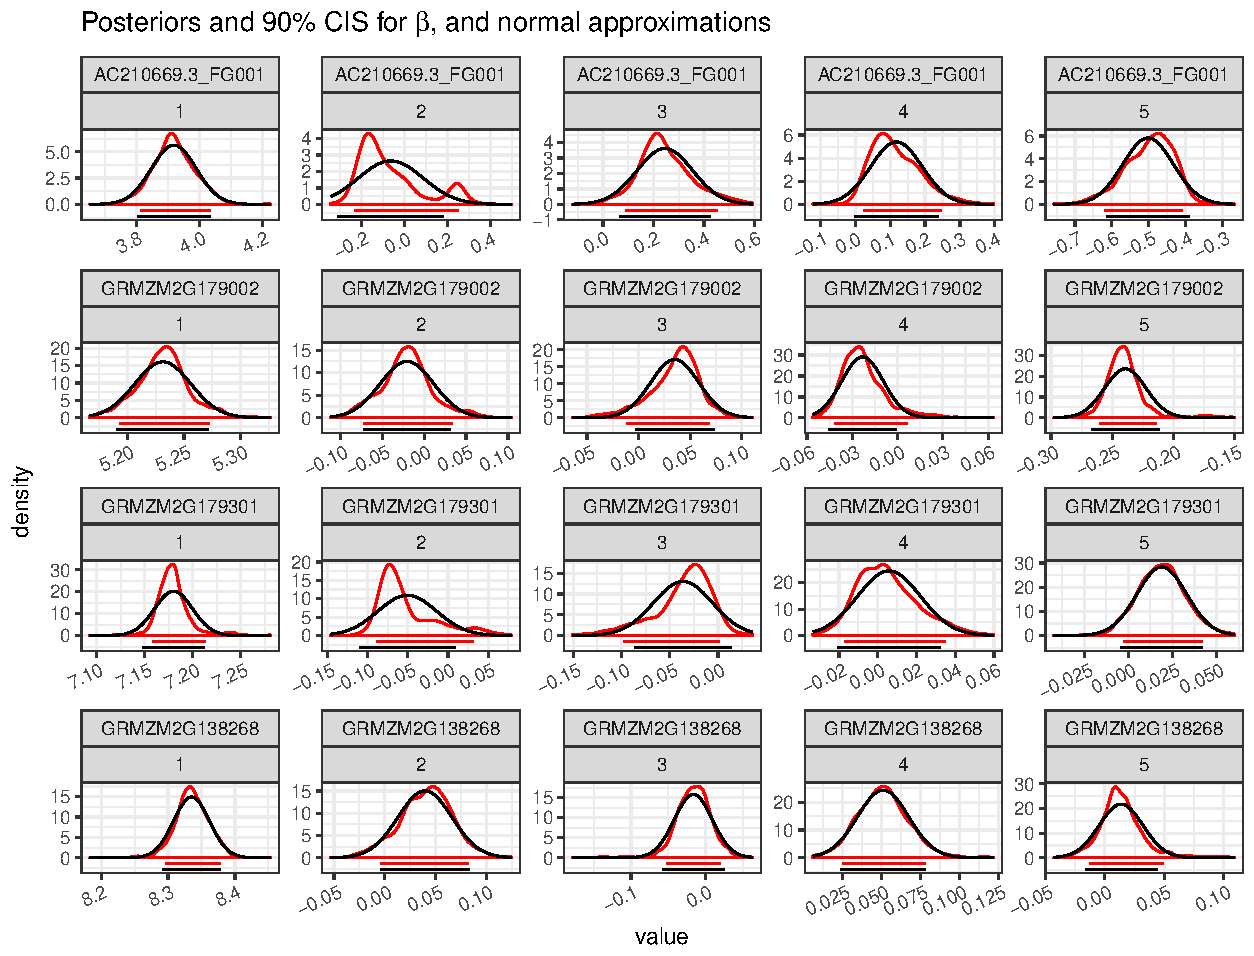
\includegraphics[width=\textwidth]{sample_genes_cis}
\begin{minipage}{.8\textwidth}
\caption{Posterior distributions of $\beta_g$ for 4 randomly selected genes (red). Normal approximations based on the first two posterior moments are also shown (black). Line segments representing 90\% credible intervals are drawn in the lower part of each plot. }
\end{minipage}
\label{compare-to-approx}
\end{figure}

\begin{figure}
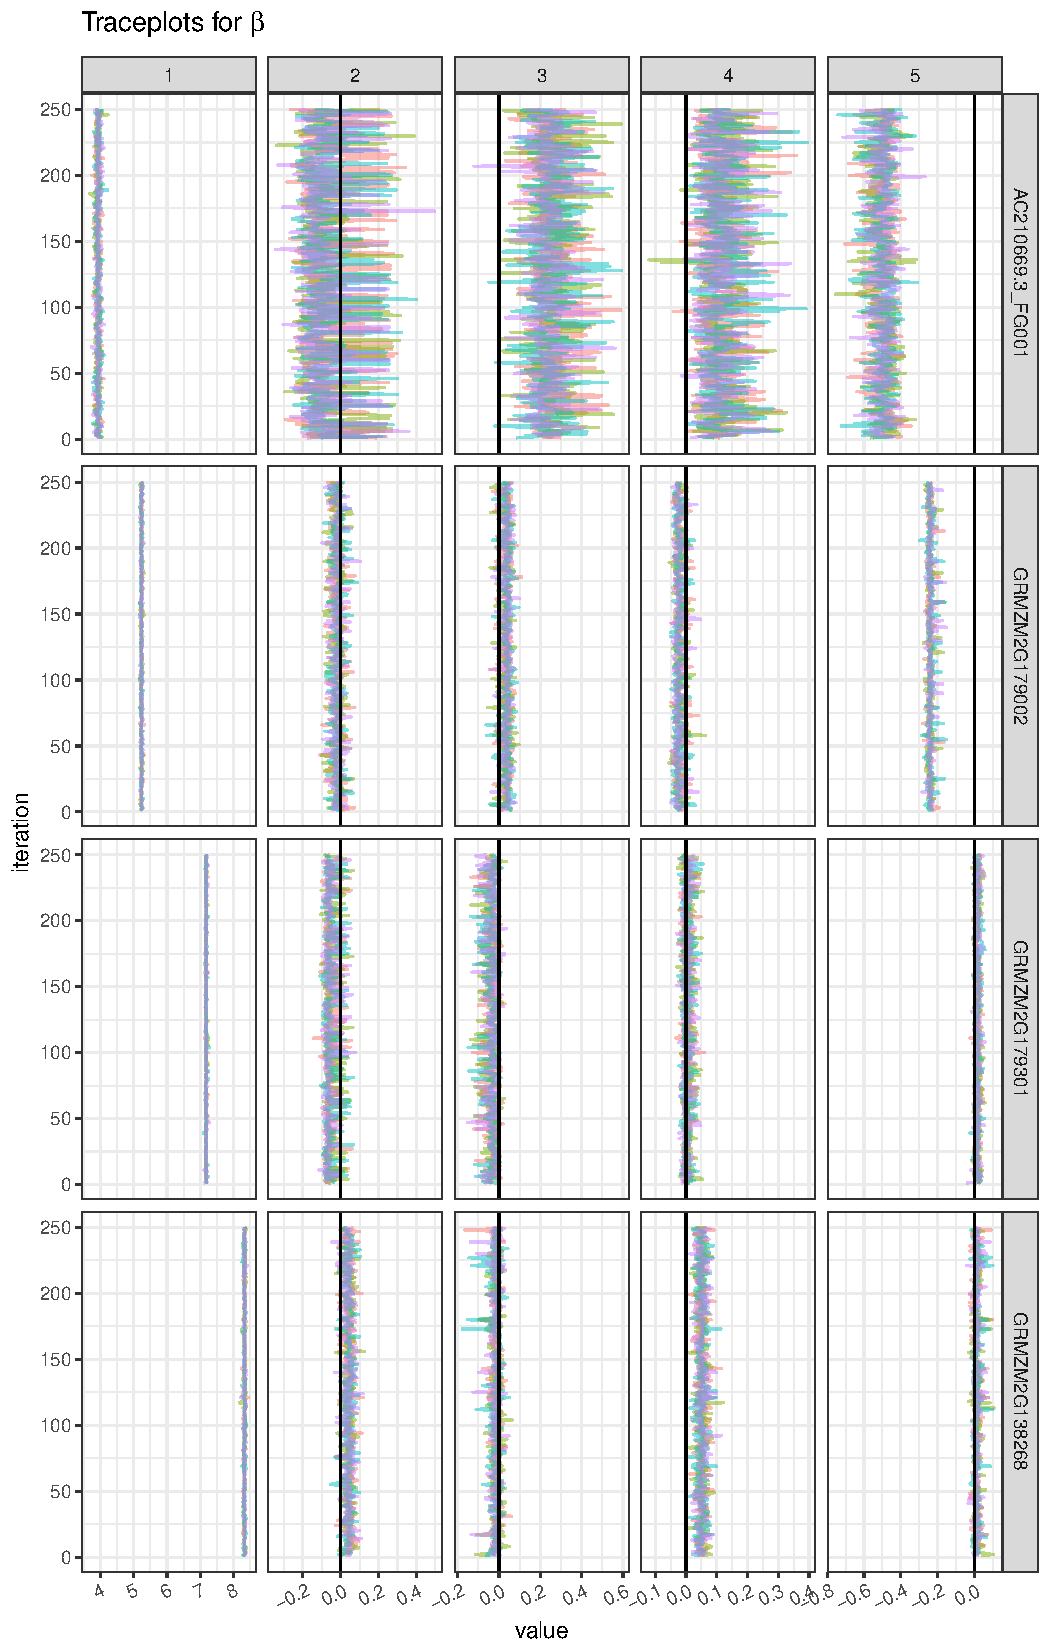
\includegraphics[width=.8\textwidth]{sample_genes_trace}
\begin{minipage}{.8\textwidth}
\caption{Traceplots of $\beta$ for randomly selected genes. 250 thinned samples for each independent Markov chain, the chain identified by color, are shown.}
\end{minipage}
\label{mixing}
\end{figure}

\begin{figure}
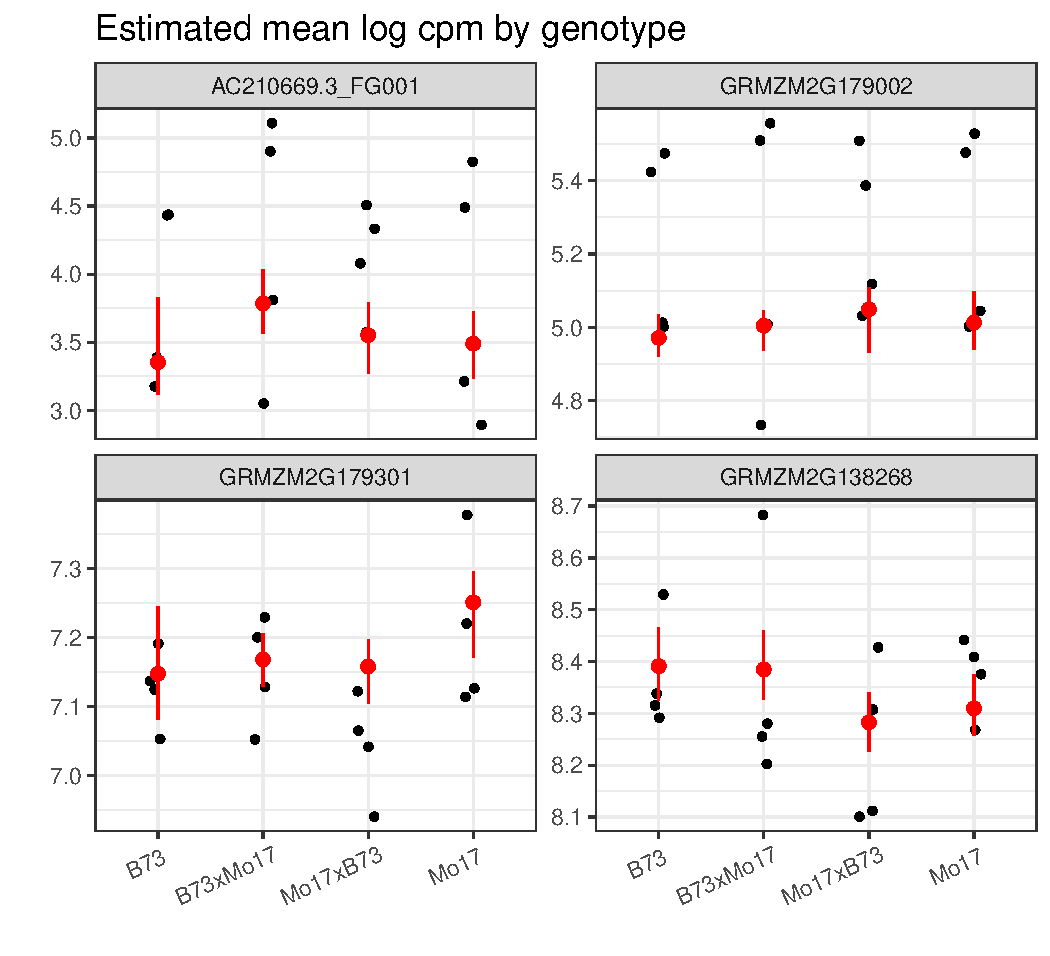
\includegraphics[width=.7\textwidth]{sample_genes_mean}
\begin{minipage}{.8\textwidth}
\caption{Adjusted log-cpm for randomly selected genes by genotype (black) and corresponding posterior means and 90\% confidence intervals for the mean expression (red).}
\end{minipage}
\label{compare-cis}
\end{figure}
}




% Thresholding by $\mu_{12} - t > \max\left\{\mu_1,\mu_2\right\} \implies \beta_3+\beta_4 > |\beta_2|$

\begin{figure}[h!]
\centering
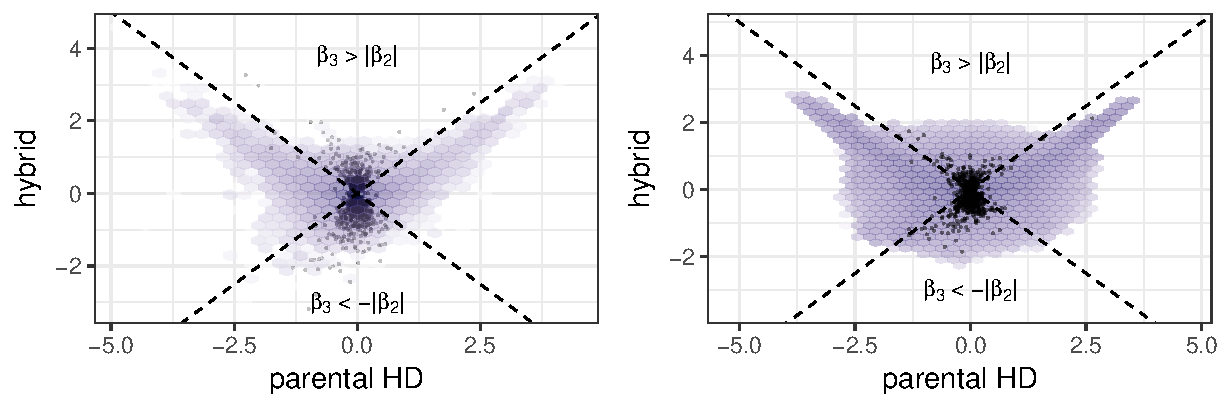
\includegraphics[width=\textwidth]{heterosis-shrinkage}
\begin{minipage}{.8\textwidth}
\caption{\small The left panel shows independently obtained estimates for the parental half-difference and the mean hybrid effect for genes classified as heterotic in Paschold et al. (2012) overlayed on a bivariate histogram of the independent estimates for all genes. The right
panel shows the corresponding estimates for our analysis overlayed on a posterior pointwise estimate of $\mathcal{P}$. In this second plot we can see significant shrinkage toward the regions where $\mathcal{P}$ puts more probability in the posterior.}
\end{minipage}
\label{het-shrink}
\end{figure}

\section{Discussion}
Hierarchical models have an important role in problems where, as is true in gene expression, the number of model parameters is much larger than the number of subjects. By modeling the parameters, we use the ``between-gene" information in the data to moderate our inferences about individual genes . The use of hierarchical models for gene expression analyses is standard. Empirical evidence suggests, however, that model assumptions often made about the distribution of the gene-specific parameters are not realistic --- rather, the empirical distributions can exhibit complex shapes. However, it seems difficult to suggest a parametric alternative to the common default assumptions (independence, normality.) We have demonstrated a computationally demanding, yet feasible, alternative: a Dirichlet process prior on this unknown distribution.

Our simulation studies show that the BNP methodology provides a viable alternative to more standard methods. Intuitively, we expect that it should do better than the alternative methods we considered in cases when the distribution of gene-effects has an unusual shape that contradicts independence. We can imagine situations where the underlying distribution of the gene specific parameters is itself an object of importance. For example, the v-shape displayed in Figure \ref{het-shrink} describes a pattern whereby the average hybrid mean expression tends toward but generally remains less than the mean expression of the higher parent. We might interpret this to be a result of dominance, where a dominant allele masks the affect of the recessesive allele in the heterozygous maize plant.

When there is only interest in expression at the level of genes, it should still be valuable to have a model flexible enough to handle detectable patterns in the data. Figure \ref{all-shrink} shows side-by-side plots of the distribution of the estimated components by BNP and DESeq2, which assumes independent priors on the gene-specific effects (excluding the intercept). The BNP estimates are shrunk toward the mass of the distribution, whereas DESeq2 estimates are shrunk toward the origin.


\begin{landscape}
\centering
\begin{figure}
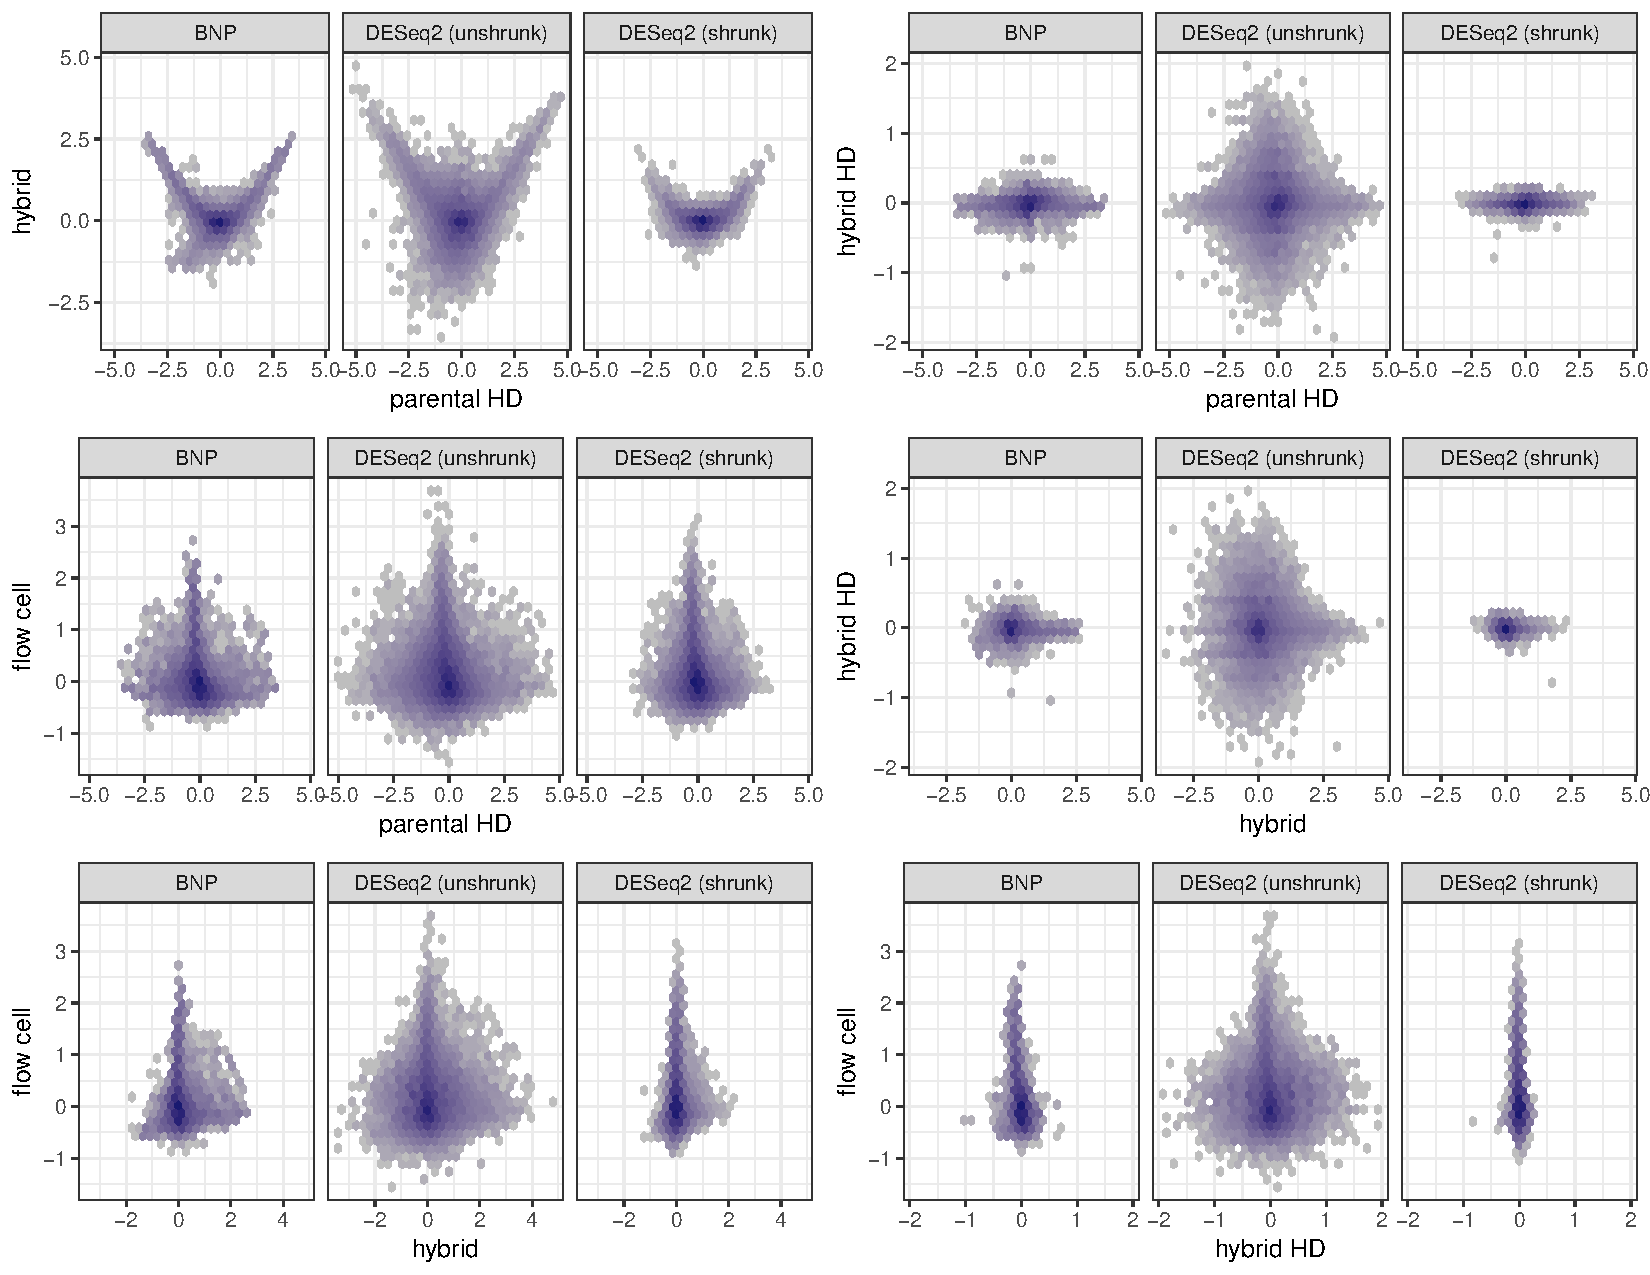
\includegraphics[height=.9\textheight]{pairs-shrinkage}
\caption{Bivariate histograms of estimates of gene-specific effects, excluding intercepts. The estimates shown are posterior means obtained with the BNP method as well as estimates obtained with DESeq2 with and without independent normal shrinkage priors (MAP and MLE, respectively) are shown.}
\label{all-shrink}
\end{figure}
\end{landscape}

Additionally, while posterior sampling is cumbersome in the amount of memory involved (approximately 6 GB for 4,000 samples of $\beta$), the interpretability of posterior quantities of interest and the inferential flexibility allowed make a strong case for the use of the Bayesian approach.



There are various modifications that might be considered to our model, within the same graphical structure. In the BNP method, precision weighting was used to correct for inaccuracies in mean-variance relationship implied by a normal assumption on the normalized log-counts. We would prefer not to have our inference conditional on these pre-computed estimates. An alternative approach would be to adopt an over-dispersed count model, such as the negative binomial and model the counts directly. Our reason for not doing this in the first place is that by proper choice of base measure, we get conditionally conjugate draws for $\tilde{\beta}_k$ and $\tilde{\sigma}^2_k$ that depend only on simple linear combinations of low-dimensional summaries of the counts. In contrast, the log-likelihood for the negative binomial involves quantities such as $\sum_n \log \Gamma(y_{gn}+\phi)$, for real-valued overdispersion parameter $\phi$, which is not linear in the parameter. Despite such nuisances, the overall structure of our Gibbs sampler would remain unchanged.

Another modification that we might consider is the choice of prior for the stick-breaking weights. The implication of the $\op{Beta}(1, \alpha)$ priors is that the weights decay exponentially on average. A generalization described in \cite{ishwaran2001} is $\nu \sim \op{Beta}(1-a, b + ak)$, which the authors refer to as a Pitman-Yor process, contains the Dirichlet process as a special case ($a=0,b=\alpha$). Other restrictions can selected to represent alternative prior assumptions. For example, one can select $a=\alpha, b=0$ which implies that the weights follow a power law. We might expect that this would lead to more significant weights and thus less aggressive shrinkage that the Dirichlet process.


